\section{Analyse préliminaire : filtrage numérique}

\subsection{Références} 
\begin{itemize}
\item Cours de Xavier Pessoles support de cours de  PSI* La Martinière Monplaisir.
\item Patrick Beynet, \textit{Supports de cours de TSI 2}, Lycée Rouvière, Toulon.
\item David Crochet (créer à partir de KmPlot), CC-BY-SA-3.0, via Wikimedia Commons \url{https://upload.wikimedia.org/wikipedia/commons/6/6f/Fourier_d\%27un_carr\%C3\%A9.svg}.
\end{itemize}


\subsection{Filtre numérique passe bas du premier ordre}
Soit un filtre linéaire du premier ordre. Son équation différentielle est de la forme :
$$
s(t)+\tau \dfrac{\text{d} s(t) }{\text{d}t} = K e(t)
$$

En utilisant un schéma d'Euler implicite, on a l'approximation suivante : $\dfrac{\text{d} s(t) }{\text{d}t} = \dfrac{s_{k}-s_{k-1}}{h}$. En conséquences, 

$$
s_k+\tau \dfrac{s_{k}-s_{k-1}}{h} = K e_k \Leftrightarrow 
s_k = \dfrac{h K e_k+\tau s_{k-1}}{h+\tau}
$$

La fréquence d'échantillonnage est ici de 1 KHz. Le pas de dérivation est de 0,001 s. On réalise alors différents filtrages en faisant varier la pulsation de coupure du filtre. 

%\begin{minipage}[c]{.43\linewidth}
%\begin{center}
%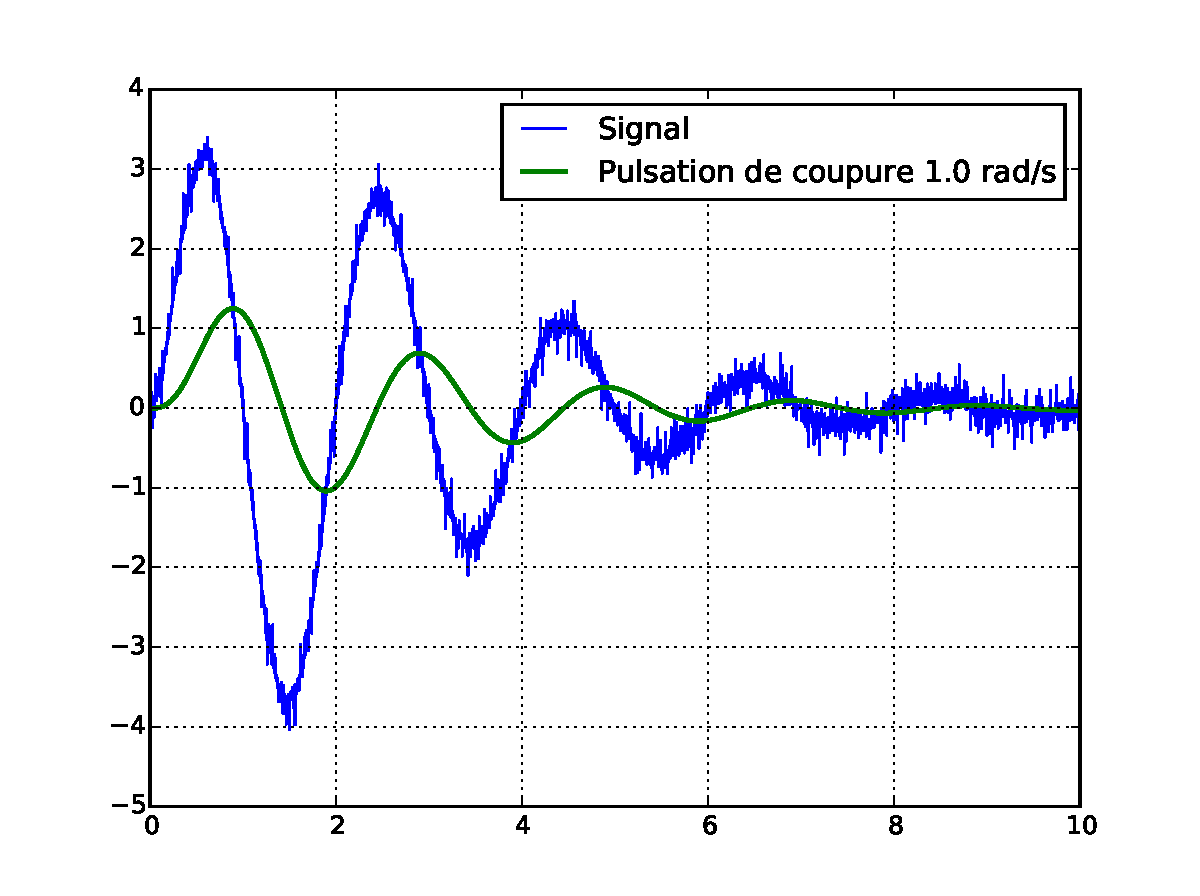
\includegraphics[width=\textwidth]{images/ordre1_1}
%\end{center}
%\end{minipage} \hfill
%\begin{minipage}[c]{.43\linewidth}
%\begin{center}
%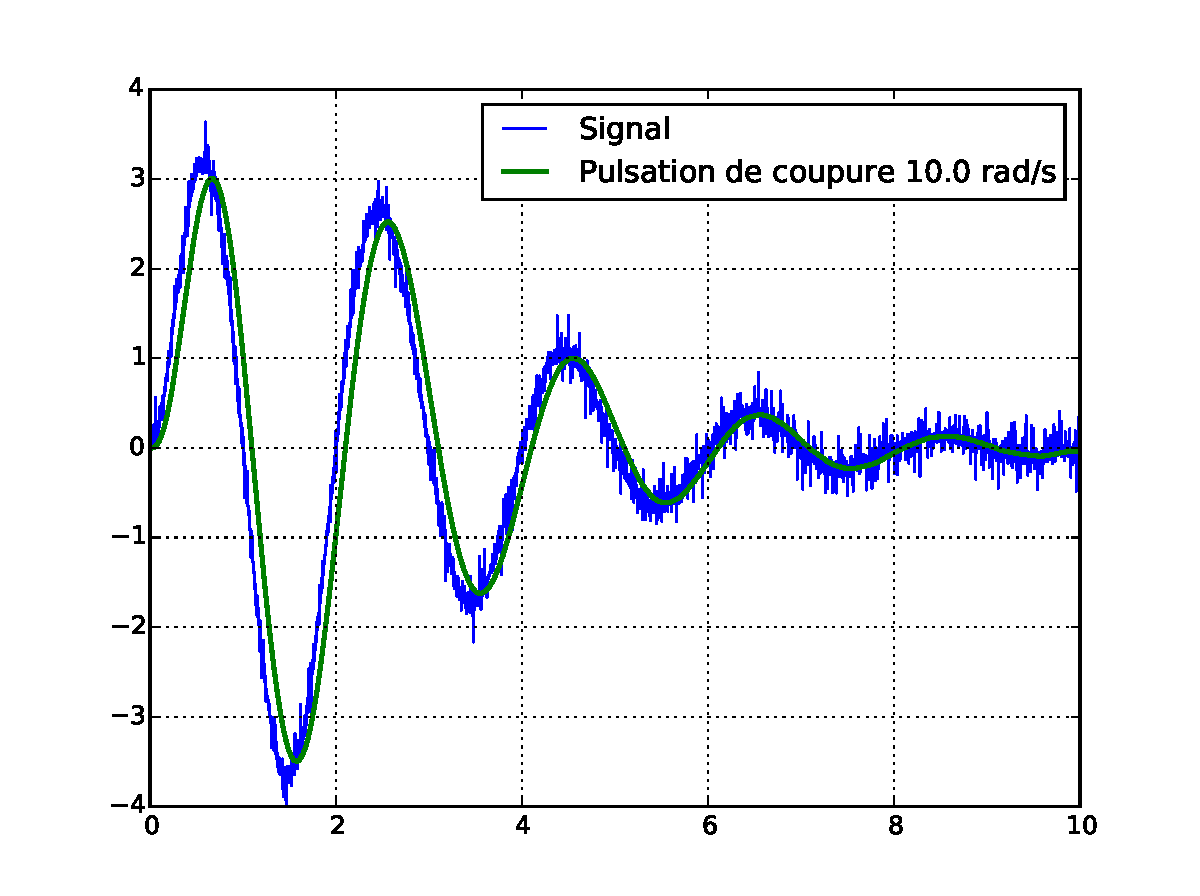
\includegraphics[width=\textwidth]{images/ordre1_2}
%\end{center}
%\end{minipage} 
%
%\begin{minipage}[c]{.43\linewidth}
%\begin{center}
%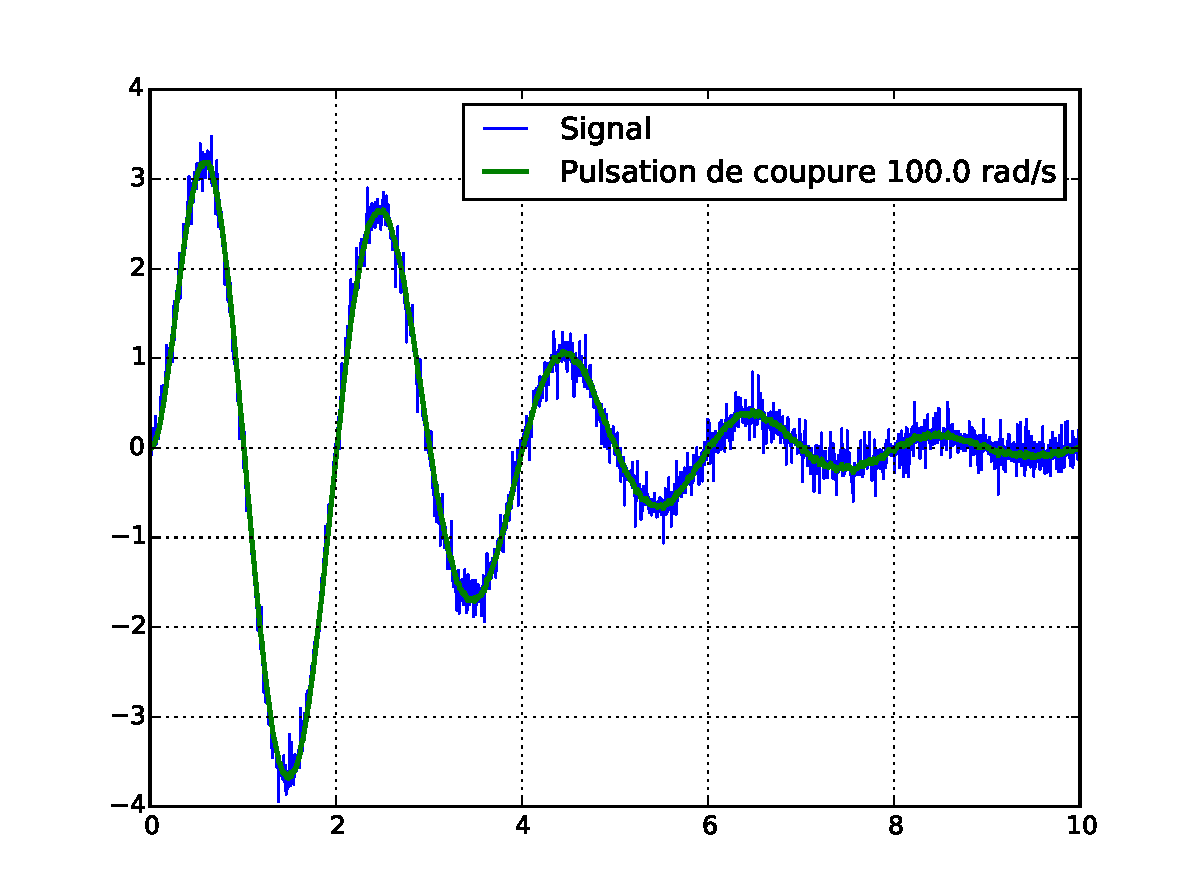
\includegraphics[width=\textwidth]{images/ordre1_3}
%\end{center}
%\end{minipage} \hfill
%\begin{minipage}[c]{.43\linewidth}
%\begin{center}
%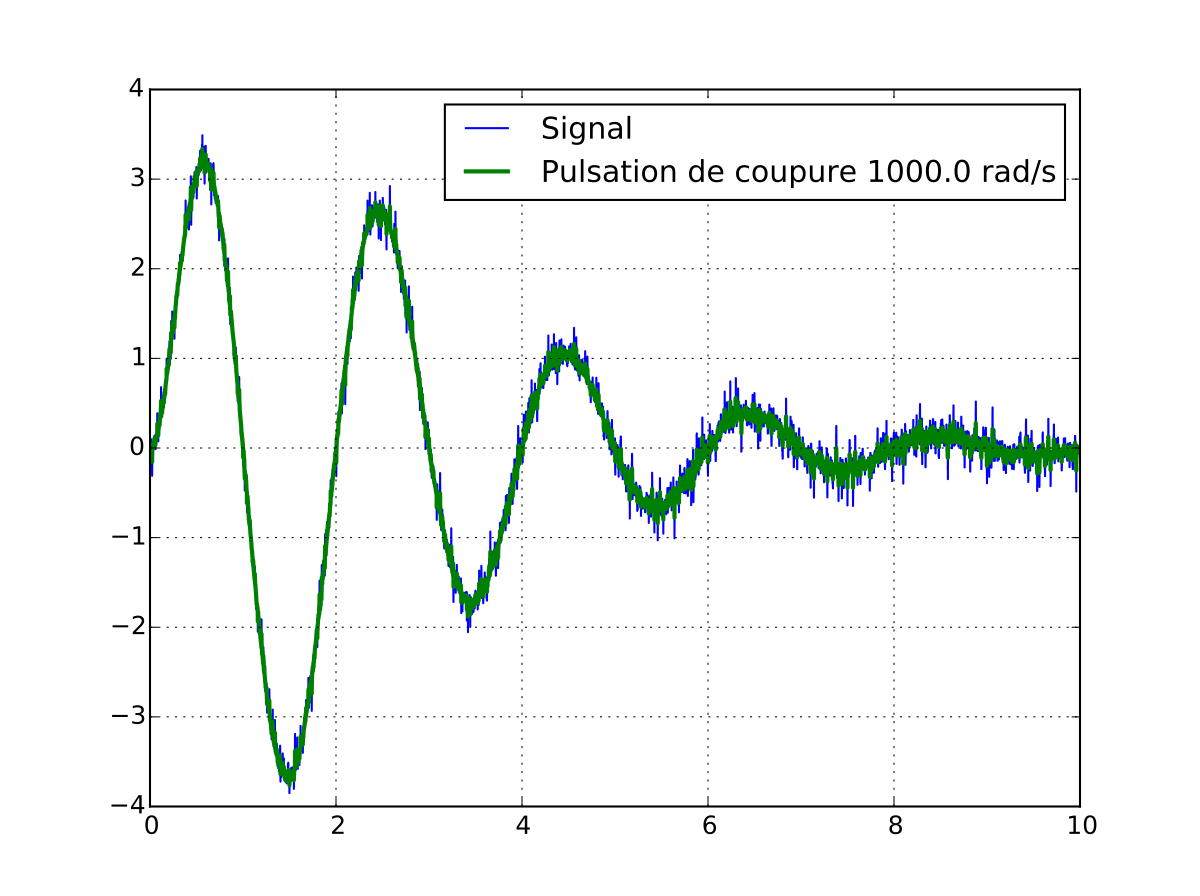
\includegraphics[width=\textwidth]{images/ordre1_4}
%\end{center}
%\end{minipage}

On observe que lorsque la pulsation de coupure diminue, le signal est de plus en plus lissé, limitant ainsi le bruit. En revanche, le signal est atténue et déphasé. 




On donne l'algorithme permettant de réaliser ce filtre à partir d'un tableau "$signal$" contenant des valeurs pour chaque instant t correspondant au tableau "$t$" avec une fréquence de coupure "$freq$".

\begin{pyverbatim}
def filtrage_passe_bas(freq,t,signal):
    tau = 1/freq # Coupure du filtre
    K=1
    res=[signal[0]]
    for i in range(1,len(signal)):
        h=t[i]-t[i-1]
        res.append((h*K*signal[i]+tau*res[-1])/(h+tau))
    return res
\end{pyverbatim}

\subsection{Filtrage numérique par moyenne glissante}
Une autre solution pour lisser une courbe est de réaliser une moyenne glissante. Si on réalise ce filtrage en temps réel, cela signifie qu'un point lissé à l'échantillon $n$ est la moyenne des $n-1$ échantillons précédents et de l'élément en cours. 

Il faut donc attendre l'acquisition de $n-1$ échantillons avant de disposer de la courbe.


%\begin{minipage}[c]{.43\linewidth}
%\begin{center}
%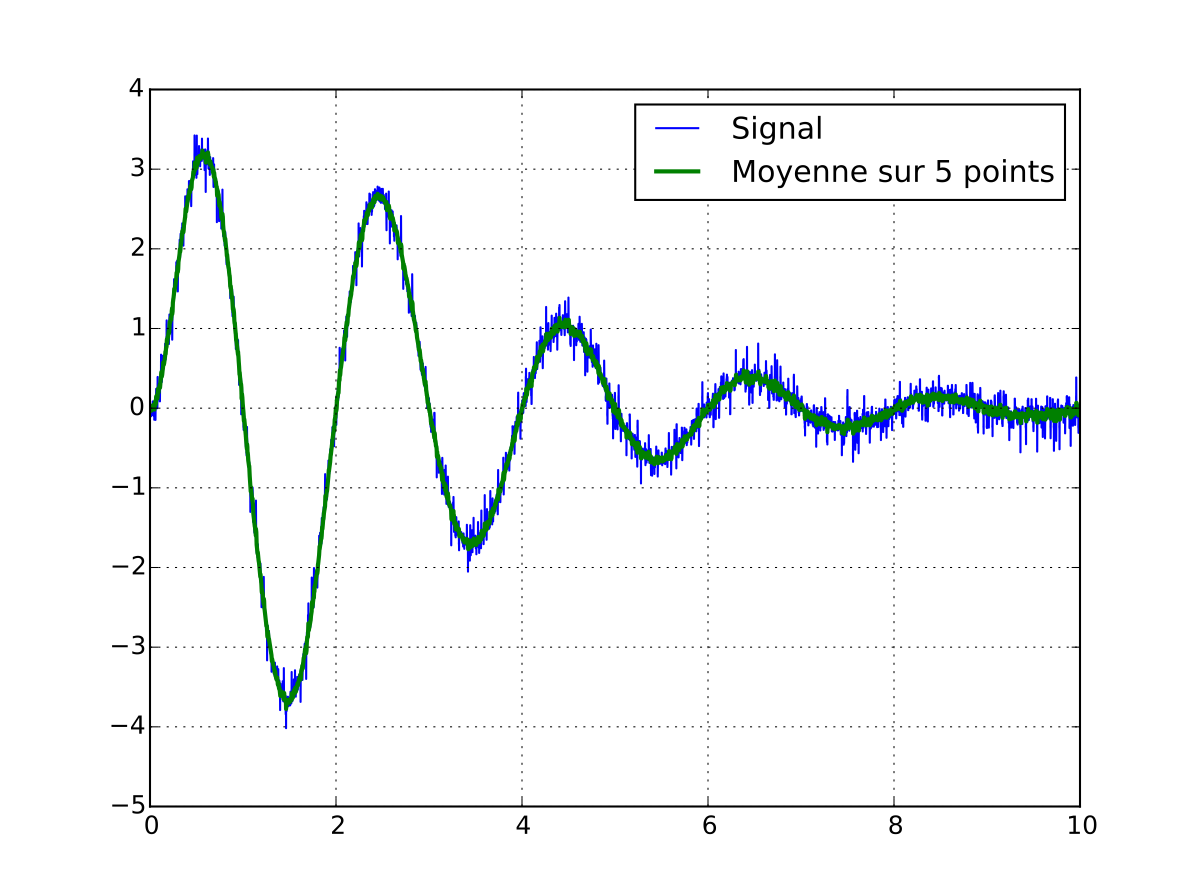
\includegraphics[width=\textwidth]{images/moyenne_1}
%\end{center}
%\end{minipage} \hfill
%\begin{minipage}[c]{.43\linewidth}
%\begin{center}
%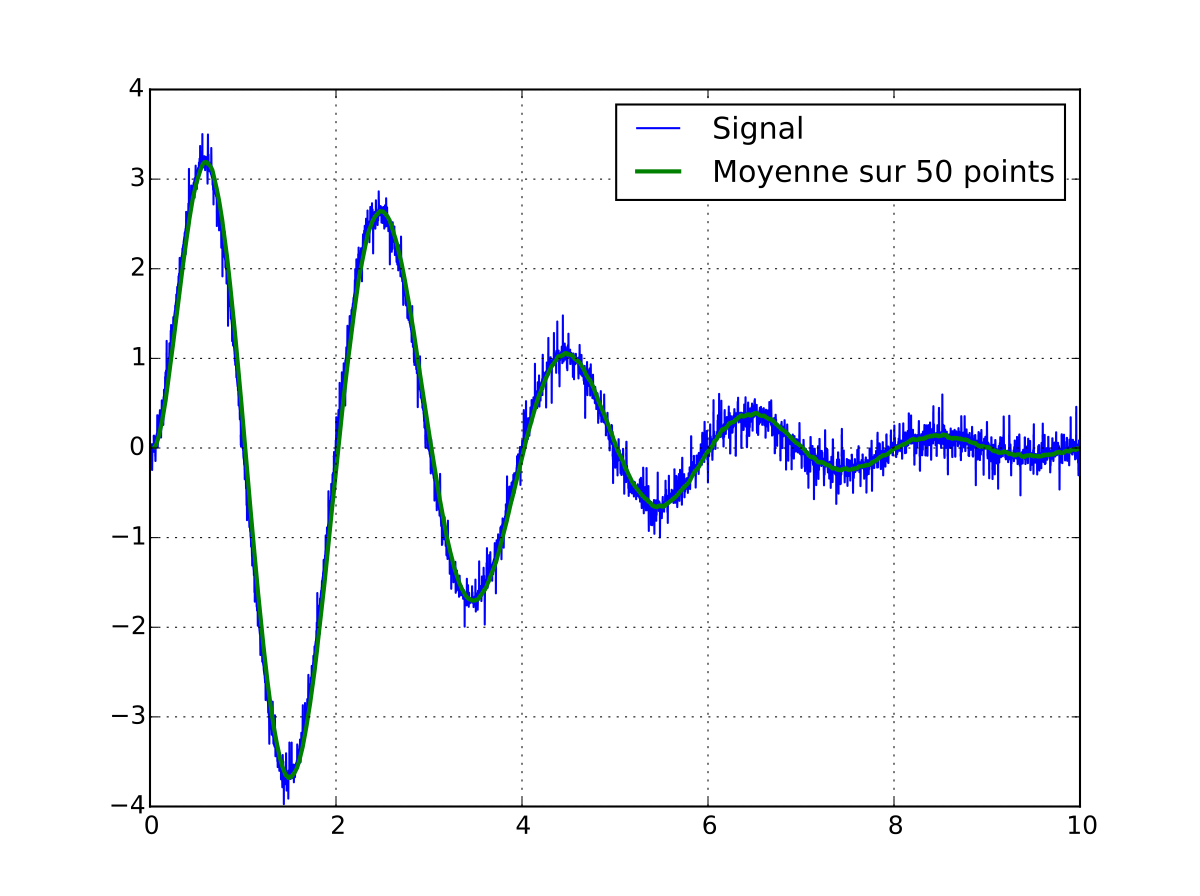
\includegraphics[width=\textwidth]{images/moyenne_2}
%\end{center}
%\end{minipage} 
%
%\begin{minipage}[c]{.43\linewidth}
%\begin{center}
%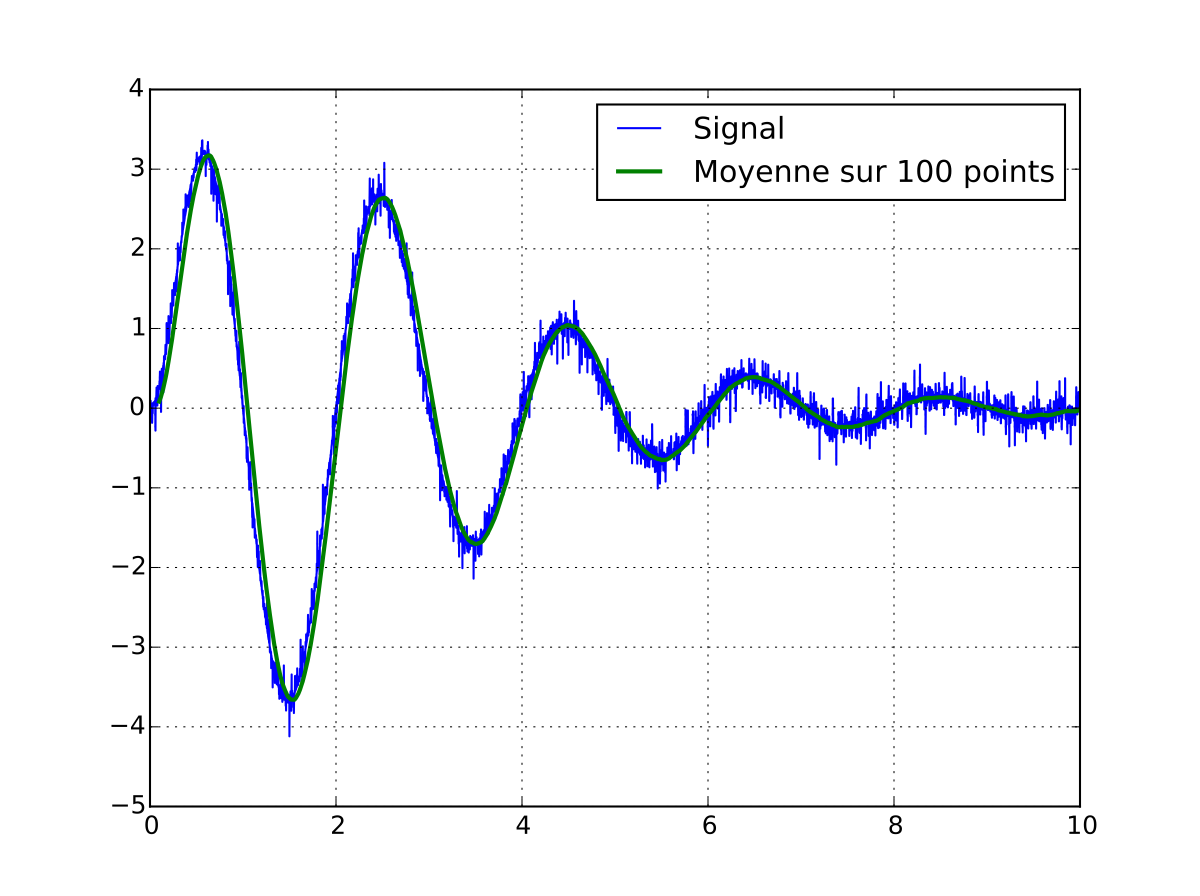
\includegraphics[width=\textwidth]{images/moyenne_3}
%\end{center}
%\end{minipage} \hfill
%\begin{minipage}[c]{.43\linewidth}
%\begin{center}
%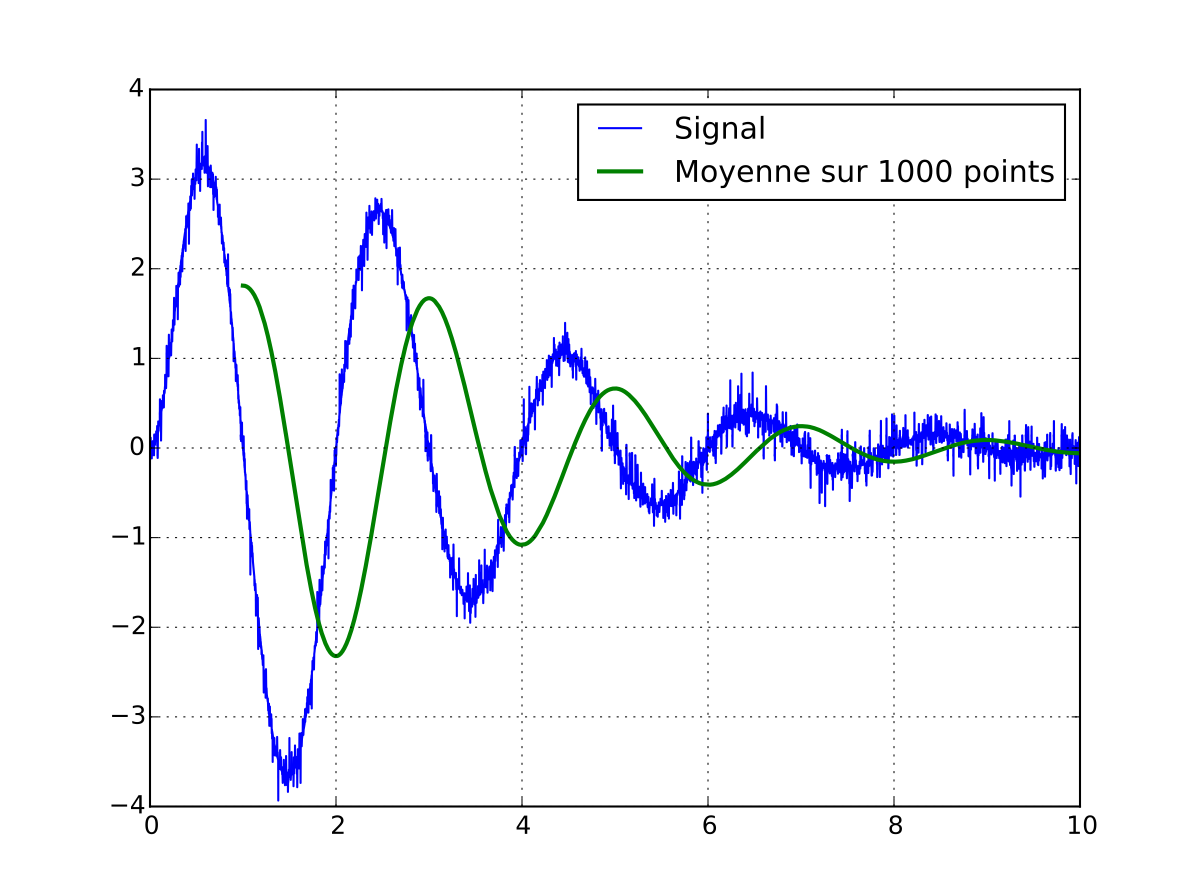
\includegraphics[width=\textwidth]{images/moyenne_4}
%\end{center}
%\end{minipage}

On donne l'algorithme permettant de réaliser ce filtre à partir d'un tableau "$signal$" contenant des valeurs pour chaque instant t correspondant au tableau "$t$" avec une taille de fenêtre de filtrage "$freq$".

\begin{pyverbatim}
def filtrage_moyenne(signal,fenetre):
    filtrageg =signal[0:fenetre-1]
    for i in range(fenetre-1,len(signal)):
        s = sum(signal[i-fenetre+1:i+1])/fenetre
        filtrageg=np.concatenate([filtrageg,np.array([s])])
    return filtrageg
\end{pyverbatim}


\section{Analyse des performances d'un cyclisme}

\subsection{Analyse d'un fichier gpx}

\subsubsection{Lecture du fichier}

\question{} Ecrire un programme permettant de savoir si un mot se trouve dans une chaine de caractère.

Un fichier gpx permet d'écrire l'ensemble des données issues d'un appareil du type gps ou montre connecté. Il recueille les 3 coordonnées spatiales (altitude par rapport au niveau de la mer, latitude et longitude) en fonction du temps. Ce fichier contient donc un ensemble de coordonnées spatiales en fonction du temps.
Ouvrir le fichier gpx et analyser son contenu.
On remarquera en particulier que le fichier est organisé d'un certaine manière. Ce fichier comporte différentes balises \footnote{source : wikipedia : \url{https://fr.wikipedia.org/wiki/GPX_(format_de_fichier)}}.

Le fichier ($<gpx>$) peut contenir :
\begin{itemize}
\item Des métadonnées ($<metadata>$), décrivant le contenu du fichier GPX par entre autre :
\begin{itemize}
\item un nom ($<name>$)
\item une description ($<desc>$)
\item l'auteur du fichier ($<author>$) comprenant son nom, une adresse mail et un lien vers son site web.
\item $\cdots$
\end{itemize}
\item Une liste de traces ou track ($<trk>$) chacune décrite par :
\begin{itemize}
\item un nom ($<name>$) ;
\item  le type d'itinéraire($<type>$)
\item des segments de trace ($<trkseg>$), le passage d'un segment à un autre indique une extinction du récepteur GPS ou une perte de réception. Un segment de trace est constitué :
\begin{itemize}
\item d'une liste ordonnée de points de trace ($<trkpt>$) dans laquelle figure respectivement la latitude ('lat') ainsi que la longitude ('long') en $^{\circ}$.
\item avec son altitude par rapport au niveau de la mer en mètres ($<ele>$)
\item un horodatage ($<time>$)
\end{itemize}
\end{itemize}
\end{itemize}

%\begin{figure}[!htb]
%\begin{center}
%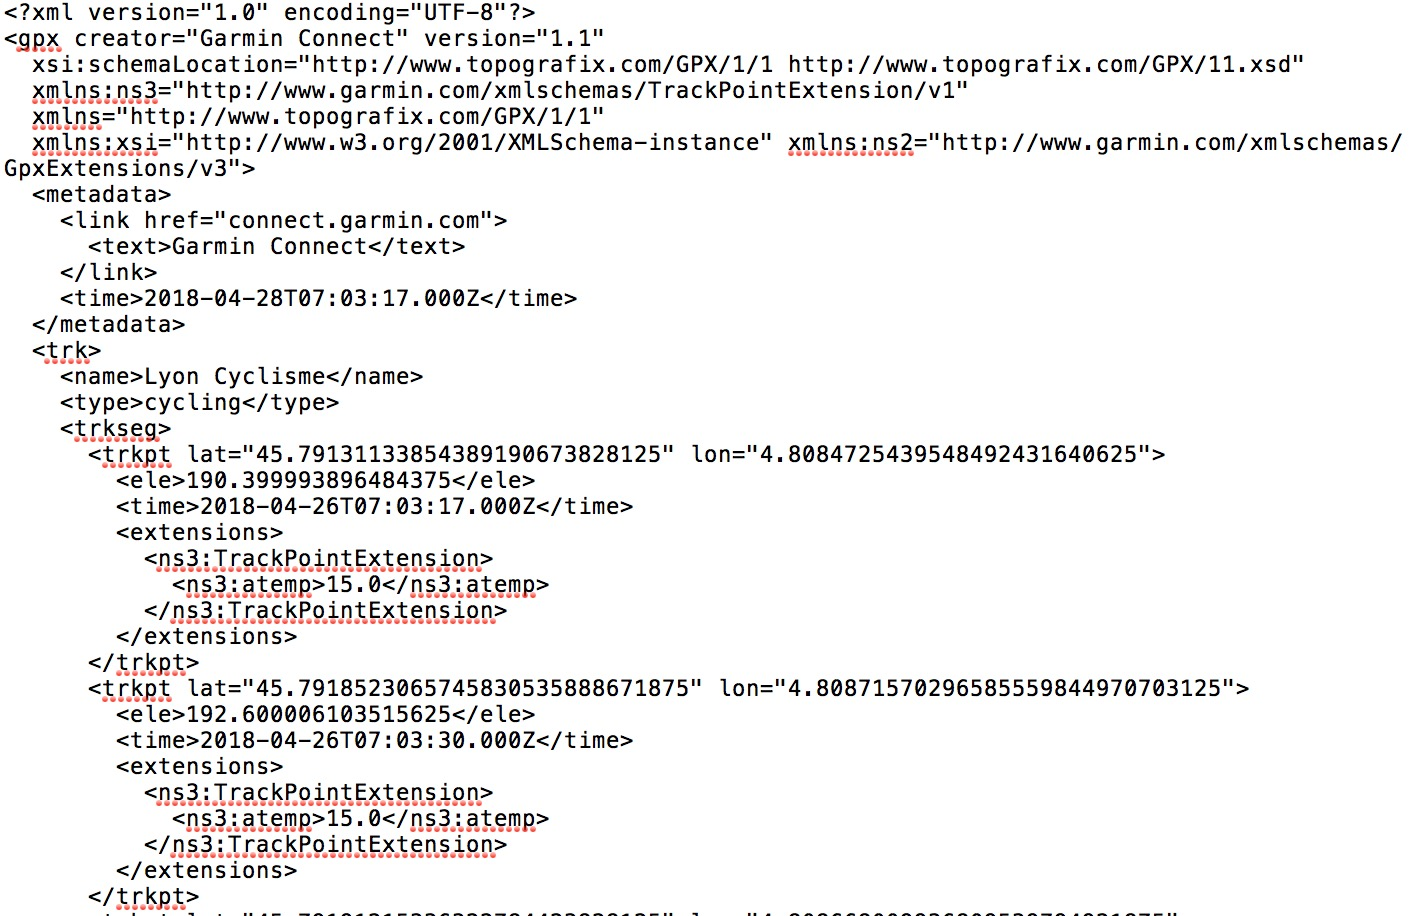
\includegraphics[width=0.8\textwidth]{fichier_gpx.jpg}
%\end{center}
%\end{figure}

\question{} Écrire un programme permettant de stocker sous la forme de 4 tableaux nommés $tp$, $lat$, $long$ et $lat$ représentant respectivement pour chaque point de mesure le temps en $s$ par rapport à l'instant initial, la latitude en $^{\circ}$, la longitude en $^{\circ}$ ainsi que l'altitude par rapport au niveau de la mer en $m$.

\subsection{Superposition du tracé sur une carte}

Pour des traces petites (comme un circuit) on peu assimiler les longitude et latitude à des coordonnées cartésiennes et il n'est donc pas nécessaire de réaliser des projections cartographiques.

\question{} A l'aide des fonctions contenues dans le module "$matplotlib.pyplot$" tracer un graphe donnant la liste des points des différentes coordonnées extraites précédemment en mettant en abscisses les valeurs de longitude et en ordonnées celles de latitude. On obtient alors la trace gps du parcours réalisé.



Pour superposer cette trace à une carte, on peut utiliser le module "$folium$" qu'il faut installer avec la commande : 

\begin{pyverbatim}
pip install folium
\end{pyverbatim}

Puis importer avec :

\begin{pyverbatim}
import folium
\end{pyverbatim}

La fonction "$Map$" permet de créer un objet carte centrée avec en point possédant une latitude et une longitude. Dans les arguments de cette fonction, il faut préciser les coordonnées en latitude et en longitude (en $^{\circ}$) ainsi le niveau d'agrandissement initial avec l'entier $z$.

\begin{pyverbatim}
macarte = folium.Map(location=[lat,long], zoom_start=z)
\end{pyverbatim}

Etant donnée une trace GPS comme celle importée précédemment, on peut connaître les latitudes min,max et les longitudes min,max qui lui correspondent. On peut se servir de ces dernière pour définir la carte initiale.

Pour superposer à cette carte la trace gps extraite précédemment on peut utiliser la fonction "$PolyLine$" qui est utilisable de la façon suivante : 

\begin{pyverbatim}
folium.PolyLine(points).add_to(macarte)
\end{pyverbatim}

Où la variable "$points$" est une liste de tuple contenant pour chaque coordonnée du fichier gpx respectivement la latitude et la longitude.

La méthode "save" appliqué à l'objet "macarte" et prenant en argument une chaine de caractère correspondante au nom du fichier "html" permet de créer une page html représentant la carte définie précédemment.

\question{} mettre en oeuvre les fonctions du module "$folium$" pour créer une page HTML superposant la trace GPS sur une carte avec un centrage et un niveau d'agrandissement satisfaisant. Vous pourrez visualiser la page créée en l'ouvrant un navigateur internet (Firefox, Google Chrome, etc...)


\subsubsection{Traitement du fichier}

On donne l'expression de la vitesse et de l'accélération en coordonnées sphérique d'un point matériel M dans son mouvement par rapport au référentiel terrestre $R_0$ : 

\begin{align*}
\overrightarrow{V}(M/R_0)=\left(\dot{r}\right)\overrightarrow{e}_r+\left(r\cdot \dot{\theta}\right)\overrightarrow{e}_{\theta}+\left(r\cdot \sin\theta\dot{\varphi}\right)\overrightarrow{e}_{\varphi}\\
\end{align*}

\begin{align*}
\overrightarrow{a}(M/R_0)=\left(\ddot{r}-r\cdot \dot{\theta}^2-r\cdot \sin^2\theta\dot{\varphi}^2\right)\overrightarrow{e}_r+\left(2*\dot{r}\dot{\theta}+r\cdot \ddot{\theta}-r\cdot \sin\theta\cos\theta\cdot \dot{\varphi}^2\right)\overrightarrow{e}_{\theta}+
\left(2 r\cos\theta\dot{\theta}\dot{\varphi}+2\dot{r}\sin\theta\dot{\varphi}+r\sin\theta\ddot{\varphi}\right)\overrightarrow{e}_{\varphi}\\
\end{align*}

On peut relier les paramètres $r$, $\theta$ et $\varphi$ aux coordonnées gps : 

\begin{align*}
\left\{
\begin{array}{c}
r=alt+R\\
\\
\theta=\dfrac{\pi}{2}-lat\\
\\
\varphi=long
\end{array}
\right.
\end{align*}

avec $R$ le rayon de la terre supposé constant et égal à $6 371km$

\question{} Écrire un programme prenant en argument un vecteur $y(t)$ dépendant du temps ainsi qu'un vecteur $t$ de mêmes longueurs et renvoyant le vecteur $dy$ correspondant à l'estimation de $\dfrac{dy(t)}{dt}$ par différence finie. On pourra la noter $dif(y,t)$.

\question{} Appliquer cette méthode pour donner des estimation de $\dfrac{dr}{dt}$, ... que pouvons-nous dire quand à la qualité de l'estimation de la dérivée.

\question{} Écrire une fonction $vitesse$ prenant en argument les tableaux $r$, $theta$ et $phi$ et renvoyant 4 tableau $Vr$, $Vtheta$ et $Vphi$ et V correspondant respectivement aux 3 coordonnées du vecteurs vitesse dans le système de coordonnées sphérique ainsi que la norme du vecteur vitesse.

\question{} Mettre en évidence à l'aide d'un tracé l'éventuelle corrélation entre la vitesse du cycliste et le profil en altitude du circuit.



\subsection{Modélisation des performances mécaniques}
\subsubsection{Modélisation de la puissance}

En considérant le cyclique comme un solide à masse ponctuelle (cela revient à négliger les effets d'inertie de la rotation des roues) on peut estimer la puissance que le cycliste doit développer en mouvement à l'aide du théorème de l'énergie cinétique : 

\begin{align*}
P_c=P_{inertie}+P_{aero}+P_{Pes}+P_{roul}
\end{align*}

\begin{itemize}
\item $P_inertie$ est la puissance que le cycliste doit développer pour vaincre les effets d'inertie et elle provient de la variation de l'énergie cinétique. 
\item $P_{aero}$ est la puissance qui résulte des effets aéronautique.
\item $P_{pes}$ est la puissance qui provient de l'action mécanique de pesanteur.
\item $P_{roul}$ est la puissance due à la résistance au roulement.
\end{itemize}

On se placera dans le référentiel terrestre supposé galiléen ($R_0$). Le cycliste ayant réalisé l'activité possède une masse $M=70kg$. On prendra l'accélération de la pesanteur $g=9,81m\cdot s^{-2}$.

\subsubsection{Puissance due à la résistance au roulement}

\begin{figure}[!htb]
\begin{minipage}{0.5\textwidth}
La puissance au roulement traduit la puissance que le cycliste doit développer pour lutter contre les effets de la résistance au roulement.
\begin{align*}
P_{roul}=Cr\times M\cdot g\times \Vert V(M/R_0)\Vert=
\end{align*}
Avec,
\begin{itemize}
\item $Cr$ le coefficient de roulement qui dépend de la pression dans les pneumatiques sachant qu'en condition de cyclisme de sur route les pneus sont gonflé à $6bars$.
\end{itemize}
\end{minipage}
\begin{minipage}{0.5\textwidth}
\begin{center}
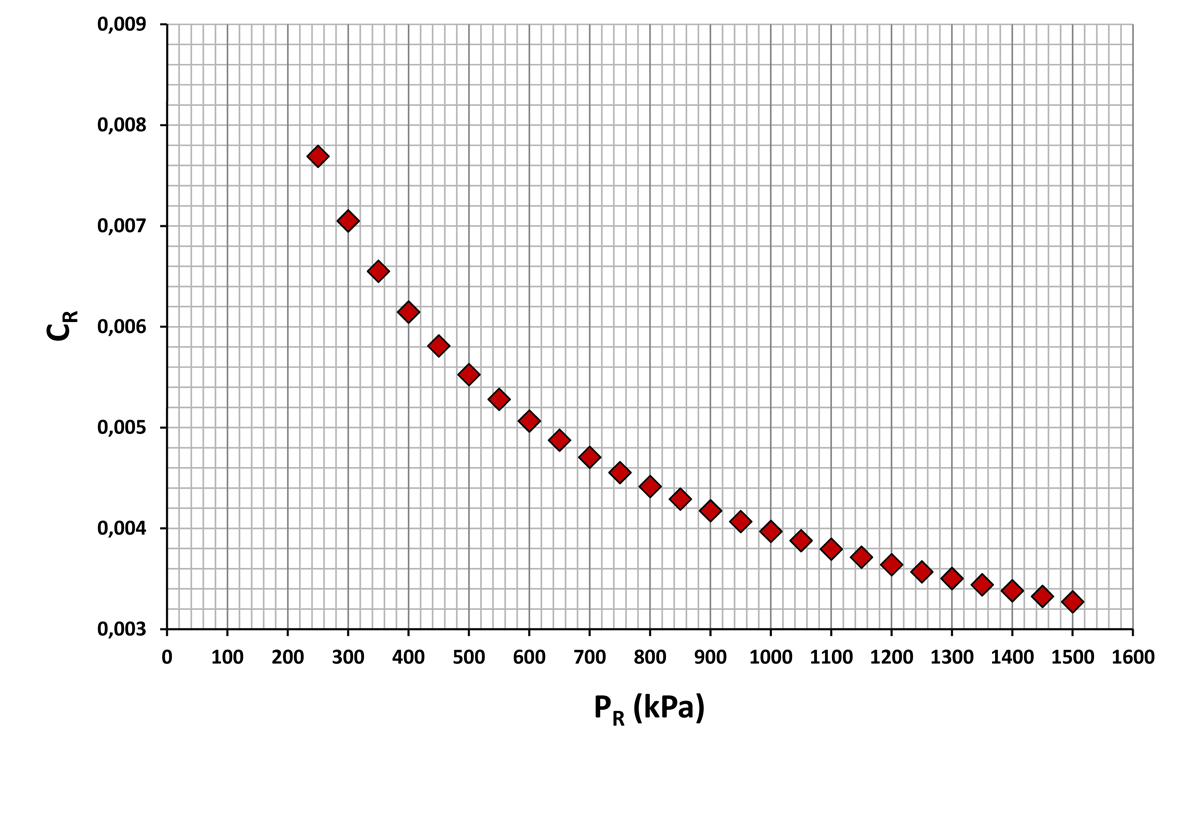
\includegraphics[width=0.9\textwidth]{resistance_roulement.png}
\caption{\label{res_roul}}
\footnote{\url{https://www.sci-sport.com/dossiers/methodes-d-evaluation-de-l-aerodynamisme-en-cyclisme-002.php}} 
\end{center}
\end{minipage}
\end{figure}

\question{} Déterminer une fonction Proul qui prend en argument la masse d'un cycliste, un vecteur V comprenant la norme de la vitesse de déplacement du cycliste ($V=\Vert \overrightarrow{V}(M/R_0)\Vert$) associé à une trace GPX, la pression dans les pneus et qui renvoie la puissance instantanée de roulement.

\subsubsection{Puissance due aux effets d'inertie}

La puissance due aux effets d'inerte peut s'estimer de la façon suivante : 

\begin{align*}
P_{inertie}=M\cdot V\cdot \frac{dV}{dt}
\end{align*}

\question{} Déterminer une fonction $Pinertie$ prenant en arguments la masse d'un cycliste, un vecteur V comprenant la norme de la vitesse de déplacement du cycliste ($\Vert V(M/R_0)\Vert$) associé à une trace GPX, la pression dans les pneus et qui renvoie la puissance instantanée de roulement.

\subsubsection{Puissance aéronautique}


\begin{figure}[!htb]
\begin{minipage}{0.5\textwidth}
A la date correspondant aux données "gpx", Météo France donne les grandeurs liées au vent suivantes :
\begin{itemize}
\item Direction du vent : $\alpha_v=360^{\circ}$ (vent du nord)
\item Vecteur direction du vent : $\overrightarrow{u}_v=\cos\theta_v\overrightarrow{e}_{\theta}+\sin\theta_v\overrightarrow{e}_{\varphi}$
\item Vitesse du vent : $V_v=4,8m/s$
\item L'aire projeté du cycliste $A_p$.
\item Coefficient de trainée aérodynamique $C_d$.
\item Dans cette étude on prendra 
\end{itemize}

\begin{align*}
P_{vent}=\dfrac{1}{2}\rho\cdot A_p\cdot C_d\cdot V_v^2\cdot \overrightarrow{u}_v\cdot \overrightarrow{V}(M/R_0)
\end{align*}
\end{minipage}
\begin{minipage}{0.5\textwidth}
\begin{center}
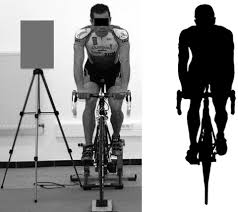
\includegraphics[width=0.9\textwidth]{aire_projetee.jpg}
\end{center}
\end{minipage}
\end{figure}


\question{} Déterminer une fonction $Paero$ prenant en arguments, la vitesse du vent ($Vv$),sa direction ($\alpha_v$), le produit $C_d\times A_p$, un vecteur V comprenant la norme de la vitesse de déplacement du cycliste ($\Vert V(M/R_0)\Vert$) associé à une trace GPX et renvoyant l'estimation de la puissance aérodynamique instantanée.  

\subsubsection{Puissance due aux effets de pesanteur}

La puissance de pesanteur va dépendre du dénivelé qui correspond à la variation de la pente en fonction de la distance parcouru.

\question{} Écrire une fonction permettant de calculer l'intégrale par rapport au temps d'une fonction $f(t)$. Elle prendre en arguments deux tableaux de même dimension $f$ et $t$ et renverra l'estimation de $I=\displaystyle{\int_{t'=0}^t}f(t')dt'$ sous la forme d'un tableau ayant la même dimension que $t$ et $f$.

\question{} Utiliser cette fonction pour donner une estimation de la distance parcouru en fonction du temps que l'on notera $x$.

La pente instantanée peut s'estimer par $\dfrac{dr(t)}{dx}$.

\question{} Écrire une fonction prenant en argument les tableaux $r$ et $x$ et renvoyant l'estimation de la pente sous la forme d'un tableau de même dimension. Pour vérifier la cohérence de cette estimation tracer sur une même figure deux graphes représentant en fonction du temps $r(t)$ et $\dfrac{dr(t)}{dx}$.

La puissance de pesanteur peut s'estimer de la façon suivante : 

\begin{align*}
P_{pes}=M\cdot g \cdot \sin\arctan\left(\frac{dr(t)}{dx}\right)\cdot \Vert \overrightarrow{V}(M/R_0)\Vert 
\end{align*}

\question{} Déterminer une fonction $Ppes$ prenant en arguments, la masse du cycliste, la coordonnées $r(t)$, un vecteur V comprenant la norme de la vitesse de déplacement du cycliste ($\Vert \overrightarrow{V}(M/R_0)\Vert$) associé à une trace GPX et renvoyant l'estimation de la puissance de pesanteur instantanée.  

\subsection{Puissance totale et profile de puissance record}

\subsubsection{Puissance totale}

\question{} A l'aide des question précédente tracer en fonction du temps les différentes puissances instantanées. Estimer la puissance totale instantanée que doit fournir et la superposer sur ce graphe.

\question{} Comment interpréter les valeurs négatives. On veillera à ne pas en tenir compte pour la suite.

L'énergie dépensée sur le circuit par le cycliste peut s'estimer de la façon suivante : 

\begin{align*}
E=\displaystyle{\int_{t=0}^{t_f}P_c(t')dt'}
\end{align*}

\question{} Mettre en oeuvre la méthode des trapèze pour calculer l'énergie totale consommée par le cycliste.
Un indicateur de performance intéressant à mettre en oeuvre est le profil de puissance record.

\subsubsection{Profile de puissance record}



\begin{figure}[!htb]
\begin{minipage}{0.5\textwidth}
Le profile de puissance record permet d'évaluer les aptitudes physiques d'un cycliste \footnote{Evaluation du potentiel physique du cycliste à travers le Profil de Puissance Record, J. Pinot, F. Grappe}  : 
\begin{itemize}
\item explosivité ;
\item tolérance lactale ;
\item PMA ;
\item Seuil anaérobie ;
\item endurance.
\end{itemize}
\end{minipage}
\begin{minipage}{0.5\textwidth}
\begin{center}
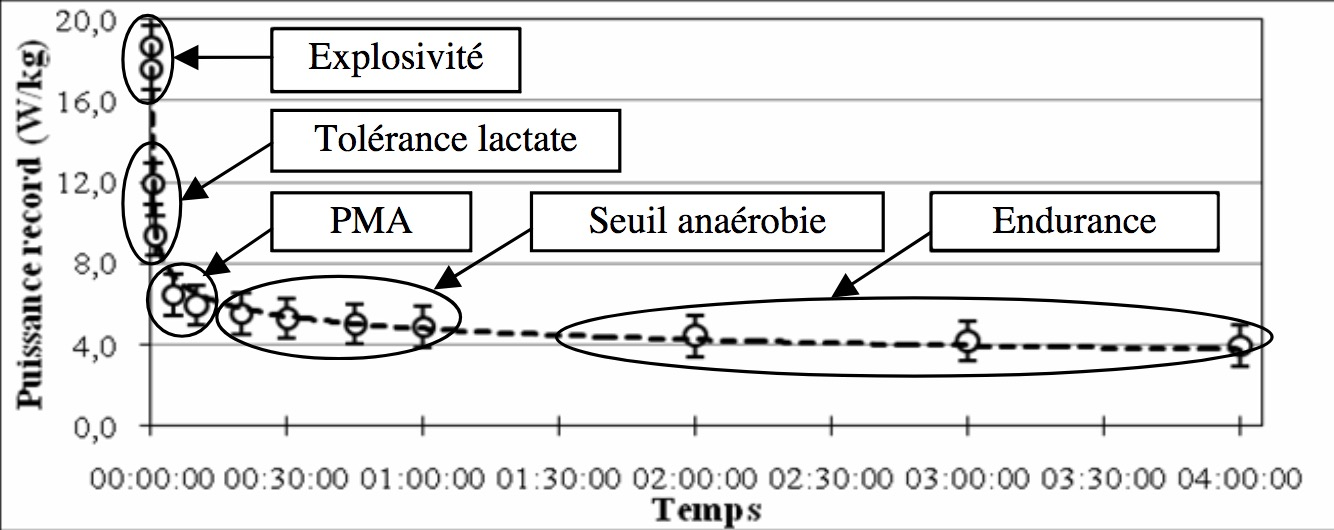
\includegraphics[width=0.9\textwidth]{PPR.jpg}
\caption{\label{PPR}}
\end{center}
\end{minipage}
\end{figure}

Il est alors intéressant pour définir le profile d'un coureur de tracer ce graphe. Pour cela il faut analyser des zone d'efforts similaire puis estimer une puissance moyenne sur la durée correspondante. On obtient alors un point sur le graphe.

\question{} A partir de l'estimation de la puissance instantanée précédente déterminer plusieurs point sur le PPR.

\section{Analyse d'une base de données de cyclistes}

\subsection{Définition des données}

La base de données étudiée comporte 3 tables : 
\begin{itemize}
\item Athlètes : comportant les caractéristiques des différents athlètes ;
\item Activités : comportant les caractéristiques des différentes activités faisant référence à des tracer gpx ;
\item Segments : faisant référence à des portion de trace gps chronométrées
\end{itemize}

\begin{minipage}{0.5\textwidth}
\begin{center}
\begin{tabular}{lllll}
\toprule
\multicolumn{5}{c}{Cyclistes}\\
\midrule
idc & nom & prenom & age & masse\\
\midrule
1&Froome&Chris&32 & 66 \\
2&Durif&Emile&23 & 70 \\
3&Bardet&Romain&27 & 65 \\
\bottomrule
\end{tabular}
\end{center}
\end{minipage}
\begin{minipage}{0.5\textwidth}
\begin{itemize}
\item \textbf{idc} : identifiant du cycliste du type \textbf{INT} ;
\item \textbf{nom} : nom du cycliste du type \textbf{VARCHAR} ;
\item \textbf{prenom} : prénom du cycliste du type \textbf{VARCHAR} ;
\item \textbf{age} : age du cycliste du type \textbf{INT} ;
\item \textbf{masse} : masse du cycliste du type \textbf{INT} ;
\end{itemize}
\end{minipage}


\bigskip

\begin{minipage}{0.5\textwidth}

\begin{tabular}{llll}
\toprule
\multicolumn{4}{c}{Activités}\\
\midrule
ida &  idc & date & fichier \\
\midrule
1&2& 2018-04-28 & mont$\_$dor.gpx \\
2&2& 2018-04-21 & mont$\_$lyonnais.gpx \\
\bottomrule
\end{tabular}
\end{minipage}
\begin{minipage}{0.5\textwidth}
\begin{itemize}
\item \textbf{ida} : identifiant de l'activité du type \textbf{INT} ;
\item \textbf{idc} : identifiant du coureur ayant effectué l'activité du type \textbf{INT} ;
\item \textbf{date} : date du début de l'activité \textbf{DATE} ;
\item \textbf{fichier} : référence du fichier gpx associé \textbf{VARCHAR} ;
\end{itemize}

\end{minipage}


\bigskip

\begin{minipage}{0.5\textwidth}

\begin{tabular}{llll}
\toprule
\multicolumn{4}{c}{Segments}\\
\midrule
ids &  idc & date & fichier \\
\midrule
1&2& 2018-04-28 & mont$\_$dor.gpx \\
2&2& 2018-04-21 & mont$\_$lyonnais.gpx \\
\bottomrule
\end{tabular}
\end{minipage}
\begin{minipage}{0.5\textwidth}
\begin{itemize}
\item \textbf{ida} : identifiant de l'activité du type \textbf{INT} ;
\item \textbf{idc} : identifiant du coureur ayant effectué l'activité du type \textbf{INT} ;
\item \textbf{date} : date du début de l'activité \textbf{DATE} ;
\item \textbf{fichier} : référence du fichier gpx associé \textbf{VARCHAR} ;
\end{itemize}

\end{minipage}



\subsection{Analyse des données}